\section{Methods \& Results}
\subsection{Data Integration}

\subsection{Results}
The posed questions are answered by creating visualizations of the integrated data. Each visualization is designed to show if there is a correlation between the inspected attributes.

\subsubsection{Are terror events dependent on the weather?}
Here, the influence of the weather on terror events is inspected. The visualizations show the number of events that took place under the specified conditions. The weather influence is measured by observing the distribution of terror events for different conditions.

The weather data contains information about the daily mean temperature and daily precipitation. The temperature is split into intervals of 10$^\circ$C beginning with $< -10^\circ$C and ending with $> 30^\circ$C. The daily precipitation is mapped to types of rain, namely: no rain, light rain, moderate rain, heavy rain and very heavy rain.

For the terror events, three aspects are chosen:
\begin{itemize}
	\item Types of terror attacks
	\item The targets of attacks
	\item The used weapons in the attacks
\end{itemize}

These three aspects are represented by the tables \texttt{TerrorAttack}, \texttt{TerrorTarget} and \texttt{TerrorWeapons}, for which only the most significant attributes are chosen, if the total number of them is too large.

\paragraph{Weather - Attack Types}
There are nine distinct attack types, which are all displayed in the visualization. Bombing is the most frequent one for each weather condition, followed by armed assault.

\begin{figure}[!ht]
\centering
    \subfloat[]{\includegraphics[width=.6\textwidth]{Rain-Attack/g2-rain0_starDiagram}}\qquad\\
    \subfloat[]{\includegraphics[width=.29\textwidth]{Rain-Attack/g2-rain01-1_starDiagram}}\qquad
    \subfloat[]{\includegraphics[width=.29\textwidth]{Rain-Attack/g2-rain11-5_starDiagram}}\qquad\\
    \subfloat[]{\includegraphics[width=.29\textwidth]{Rain-Attack/g2-rain51-20_starDiagram}}\qquad
    \subfloat[]{\includegraphics[width=.29\textwidth]{Rain-Attack/g2-rain>201_starDiagram}}
\caption{Influence of rain on terror attack types}
\end{figure}

The influence of rain on attack types is very low, as the different types are proportionally similar for each type of rain.

\newpage

\begin{figure}[!ht]
\centering
    \subfloat[]{\includegraphics[width=.28\textwidth]{Temp-Attack/g2-temp<-100_starDiagram}}\qquad
    \subfloat[]{\includegraphics[width=.29\textwidth]{Temp-Attack/g2-temp-101-0_starDiagram}}\qquad
    \subfloat[]{\includegraphics[width=.29\textwidth]{Temp-Attack/g2-temp1-100_starDiagram}}\qquad
    \subfloat[]{\includegraphics[width=.29\textwidth]{Temp-Attack/g2-temp101-200_starDiagram}}\qquad
    \subfloat[]{\includegraphics[width=.29\textwidth]{Temp-Attack/g2-temp201-300_starDiagram}}\qquad
    \subfloat[]{\includegraphics[width=.29\textwidth]{Temp-Attack/g2-temp>301_starDiagram}}
\caption{Influence of temperature on terror attack types}
\label{fig:example subfigure}
\end{figure}

The temperature has a greater influence on attack types. It can be observed that more armed assaults take place when the temperature rises.

\newpage

\paragraph{Weather - Attack Targets}
The number of distinct target types is quite large, since they can be very specific (e.g. Priest). For the analysis, the ten most representative attributes have been chosen. Different to the attack type, the target types vary more for the different conditions.

\begin{figure}[!ht]
\centering
    \subfloat[]{\includegraphics[width=.6\textwidth]{Rain-Target/g2-rain0_starDiagram}}\qquad\\
    \subfloat[]{\includegraphics[width=.29\textwidth]{Rain-Target/g2-rain01-1_starDiagram}}\qquad
    \subfloat[]{\includegraphics[width=.29\textwidth]{Rain-Target/g2-rain11-5_starDiagram}}\qquad\\
    \subfloat[]{\includegraphics[width=.29\textwidth]{Rain-Target/g2-rain51-20_starDiagram}}\qquad
    \subfloat[]{\includegraphics[width=.29\textwidth]{Rain-Target/g2-rain>201_starDiagram}}
\caption{Influence of rain on attack targets}
\end{figure}

It can be observed, that heavier rain results in a bigger number of attacks on military units, patrols and convoys.


\newpage

\begin{figure}[!ht]
\centering
    \subfloat[]{\includegraphics[width=.28\textwidth]{Temp-Target/g2-temp<-100_starDiagram}}\qquad
    \subfloat[]{\includegraphics[width=.29\textwidth]{Temp-Target/g2-temp-101-0_starDiagram}}\qquad
    \subfloat[]{\includegraphics[width=.29\textwidth]{Temp-Target/g2-temp1-100_starDiagram}}\qquad
    \subfloat[]{\includegraphics[width=.29\textwidth]{Temp-Target/g2-temp101-200_starDiagram}}\qquad
    \subfloat[]{\includegraphics[width=.29\textwidth]{Temp-Target/g2-temp201-300_starDiagram}}\qquad
    \subfloat[]{\includegraphics[width=.29\textwidth]{Temp-Target/g2-temp>301_starDiagram}}
\caption{Influence of temperature on attack targets}
\label{fig:example subfigure}
\end{figure}

Lower temperatures have a high number of attacks on military personnel. With increasing temperature, this shifts towards civilians. Therefore, with higher temperature, more civilians but less military personnel are attacked. 

\newpage

\paragraph{Weather - Attack Weapon}
There are, like attack targets, many distinct attack weapons. Again, the ten most representative attributes have been chosen. The weapons have a high correlation to the attack types, seen by the attributes \texttt{Bombing/Explosion \& Unknown explosive type} and \texttt{Armed assault \& Unknown gun type}.

\begin{figure}[!ht]
\centering
    \subfloat[]{\includegraphics[width=.6\textwidth]{Rain-Weapon/g2-rain0_starDiagram}}\qquad\\
    \subfloat[]{\includegraphics[width=.29\textwidth]{Rain-Weapon/g2-rain01-1_starDiagram}}\qquad
    \subfloat[]{\includegraphics[width=.29\textwidth]{Rain-Weapon/g2-rain11-5_starDiagram}}\qquad\\
    \subfloat[]{\includegraphics[width=.29\textwidth]{Rain-Weapon/g2-rain51-20_starDiagram}}\qquad
    \subfloat[]{\includegraphics[width=.29\textwidth]{Rain-Weapon/g2-rain>201_starDiagram}}
\caption{Influence of rain on terror attack weapons}
\end{figure}

Similar to the attack types, the influence of rain  on the used weapons can hardly be seen.


\newpage

\begin{figure}[!ht]
\centering
    \subfloat[]{\includegraphics[width=.28\textwidth]{Temp-Weapon/g2-temp<-100_starDiagram}}\qquad
    \subfloat[]{\includegraphics[width=.29\textwidth]{Temp-Weapon/g2-temp-101-0_starDiagram}}\qquad
    \subfloat[]{\includegraphics[width=.29\textwidth]{Temp-Weapon/g2-temp1-100_starDiagram}}\qquad
    \subfloat[]{\includegraphics[width=.29\textwidth]{Temp-Weapon/g2-temp101-200_starDiagram}}\qquad
    \subfloat[]{\includegraphics[width=.29\textwidth]{Temp-Weapon/g2-temp201-300_starDiagram}}\qquad
    \subfloat[]{\includegraphics[width=.29\textwidth]{Temp-Weapon/g2-temp>301_starDiagram}}
\caption{Influence of temperature on terror attack weapons}
\label{fig:example subfigure}
\end{figure}

As the armed assaults increase with temperature, the number of guns used increases as well.
